\documentclass{article}
\usepackage{graphicx, mathtools, amssymb, amsmath, dirtytalk}
\graphicspath{{Images/}}

\setlength{\oddsidemargin}{0in}
\setlength{\textwidth}{6.5in}
\setlength{\topmargin}{-.55in}
\setlength{\textheight}{9in}
\pagestyle{empty}


\title{Scientific Computation II Midterm}
\author{Michael Nameika}
\date{March 2023}

\begin{document}

\maketitle

\section*{Exercise 1}
Describe and implement a fourth-order Runge-Kutta and Fourier method for the Burger equation with periodic boundary conditions:
\[u_t = \epsilon u_{xx} + uu_{x}, \:\:\:\:\: x \in (-\pi, \pi), \:\:\:\:\:u(x,0) = e^{-10\sin^2(x/2)},\]
with $\epsilon = 0.03$ and the simulation running up to $t = 1$.
\newline\newline
Recall that we can relate the spacial derivative of a function to its Fourier transform:
\[u_x = \mathcal{F}^{-1}(ik\mathcal{F}(u))\]
and similarly for the second derivative:
\[u_{xx} = \mathcal{F}^{-1}(-k^2\mathcal{F}(u))\]
That is, we may use this to transform this equation to a PDE that involves the Fourier transform of $u$:
\[\mathcal{F}(u)_t = -\epsilon k^2 \mathcal{F}(u_k) + ik \mathcal{F}\left(\frac{1}{2}u^2\right)\]
Implementing this in \verb+MATLAB+ with the fourth order Runge Kutta method (see attached \verb+scicompMidTerm1_NAMEIKA.m+ file), we find the following solution plot for $t \in [0,1]$:
\begin{center}
    \includegraphics[scale = 0.35]{burgereqRK4}
    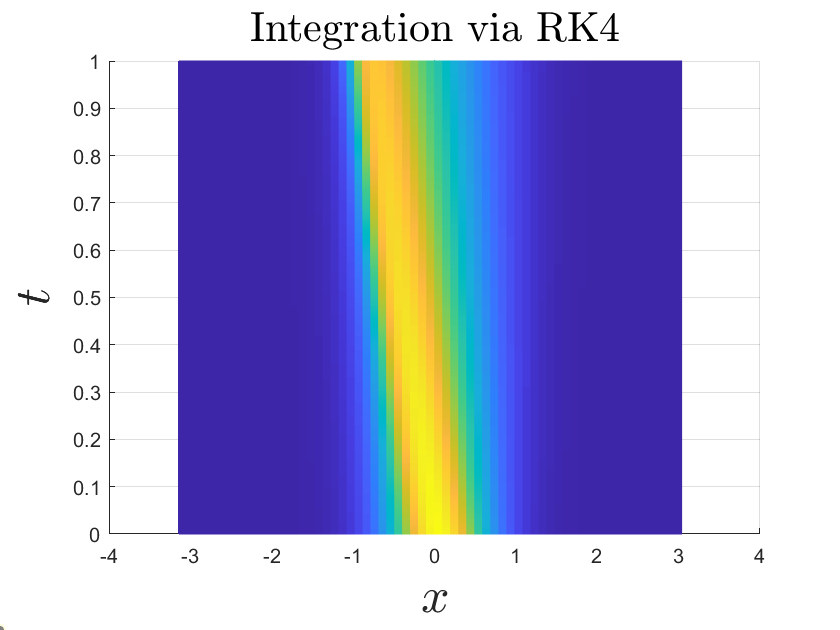
\includegraphics[scale = 0.35]{burgereqRK4TOPVIEW}
\end{center}

\section*{Exercise 2}
Consider Fisher's equation
\[u_t = u_{xx} + u(1 - u)\]
\begin{itemize}
    \item[(i)] The only traveling \say{front} wave $u(x,t) = \phi(x - ct)$ with $\phi(-\infty) = 1$ and $\phi(+\infty) = 0$ is given by
    \[u(x,t) = \left[1 + exp\left(\frac{x}{\sqrt{6}} - \frac{5}{6}t\right)\right]^{-2}\]
    Verify this assertion by deriving the ODE that $\phi$ has to satisfy and then use a numerical method to solve it. [Of course you should also try to solve it analytically!]
    \newline\newline
    Let $z = x - ct$ so that $\phi(x - ct) = \phi(z)$. Notice that $\phi_t(x - ct) = -c\phi'(z)$ and $\phi_{xx}(x - ct) = \phi''(z)$. Then our PDE ($\phi_t = \phi_{xx} + \phi(1 - \phi)$ becomes 
    \[-c\phi'(z) = \phi''(z) + \phi(z)(1 - \phi(z))\]
    Let $\psi = \phi'$ so we can write the above ODE as a system of two coupled ODEs:
    \[\frac{d}{dz}\begin{bmatrix}
        \phi\\
        \psi
    \end{bmatrix} = 
    \begin{bmatrix}
        \psi\\
        -c\psi - \phi(1 - \phi)
    \end{bmatrix}\]
    with $c = 5/\sqrt{6}$. Implementing this ODE system in \verb+MATLAB+ with initial conditions of $\psi_0 = 0$, $\phi_0 = 0.99$ (with $\psi_0 = \psi(-L), \phi_0 = \phi(-L)$, $L = -20$), we find the following plot with the exact solution plotted on the same axis:
    \begin{align*}
        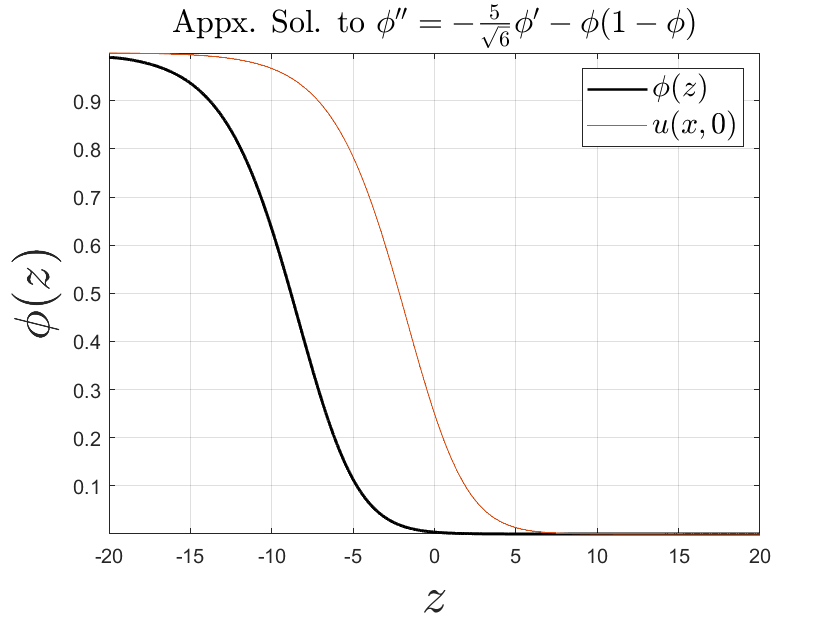
\includegraphics[scale = 0.4]{numApprox}
    \end{align*}
    Notice the similarities of the shape. Clearly, they are not exactly the same, due to needing to truncate the domain of the approximate solution, but are very similar. For additional details, see the \verb+fisherODE.m+ file.
    
    \item[(ii)] Since $u(x,t) \to 0$ (resp. 1) as $x \to +\infty$ (resp. $-\infty$), we can approximate the traveling wave given in (i) in $(-L,L)$ where $L$ is large enough so that the wave front does not reach the boundary $x = L$, by imposing the boundary conditions
    \[u(-L,t) = 1, \:\:\: u(L,t) = 0,\]
    and taking the initial value as $u(x,0)$. Design and implement a Chebyshev collocation method to approximate the solution of the PDE and study the convergence of the approximate solution as $N$ is increasing.
    \newline\newline
    To begin, since Chebyshev collocation is done on the interval $(-1,1)$, we must transform our problem from $(-L,L)$ to $(-1,1)$. Use the transformation $y \mapsto x/L$. Then
    \[u_{yy}(y,t) = \frac{1}{L^2}u_{xx}(x,t)\]
    Additionally, we must cut the interval at some large number $L$ so that we can impose our boundary conditions. For this problem, I chose $L = 20$ and so we have $u(-20,t) = 1$, $u(20, t) = 0$ In the variable $y$, $u(y,t)|_{y=-1} = 1$, $u(y,t)|_{y=1} = 0$. Implementing this into MATLAB with an Euler time step (see attached \verb+scicompMidterm2_NAMEIKA.m+ file), we find the following solution plot for $0 \leq t \leq 5$:
    \begin{center}
        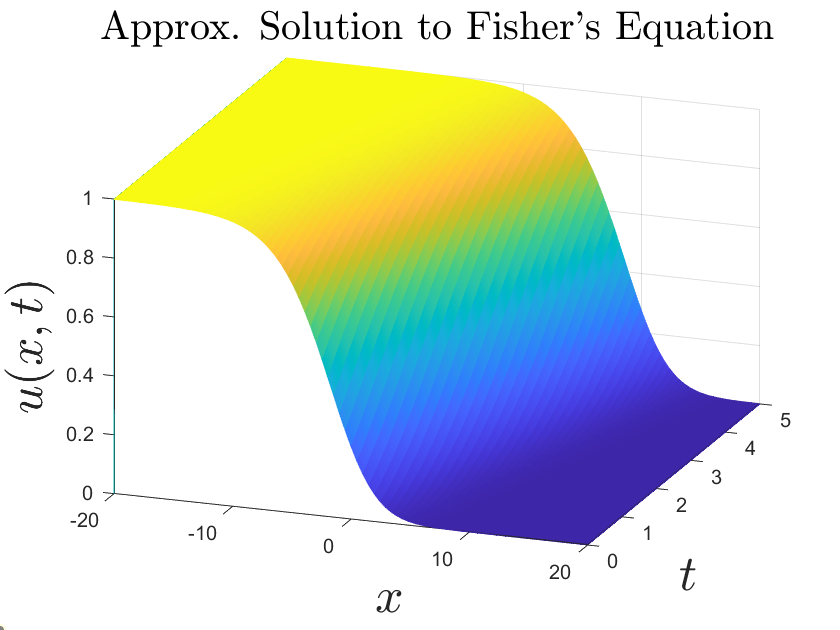
\includegraphics[scale = 0.3]{FishersEqSol}
        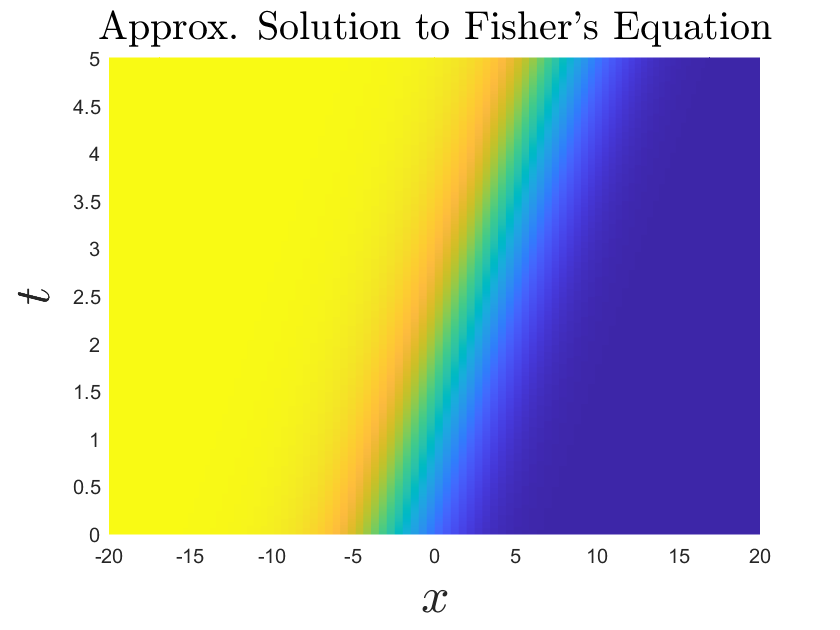
\includegraphics[scale = 0.3]{fishersTopDown}
    \end{center}
    For the maximum error between the approximate solution and the exact solution, we find the following:
    \begin{center}
        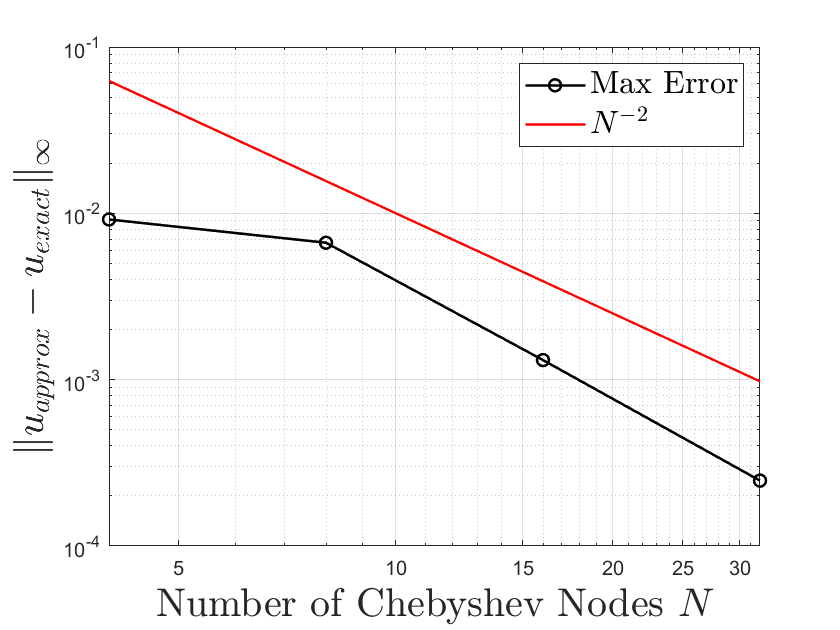
\includegraphics[scale = 0.3]{errProbii}
    \end{center}
    Increasing the number of spacial points, the error levels out at the final value in the plot above. I suspect that the reason for this is that we hit the error between the exact solution and the imposed boundary conditions of the approximate solution. In fact, that's what we can see in the below screenshot. 
    \begin{center}
        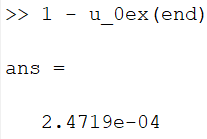
\includegraphics[scale = 0.7]{boundaryError}
    \end{center}
    I also suspect that we only see approximately 2nd order accuracy due to the Euler time stepping method. 
    
\end{itemize}

\section*{Exercise 3}
Try to accomplish as many of the tasks as in exercise 2 as you can for the FitzHugh-Nagumo system
\[u_t = u_{xx} + u(1 - u)(u - a) - v; \:\:\:\:\: v_t = \epsilon(u - bv)\]
Using the initial conditions 
\[v(x,0) = \frac{1}{2}e^{-\frac{1}{2}(x - 1/5)^2}; \hspace{2cm} u(x,0) = \frac{1}{4}e^{-\frac{1}{2}(x + 1/5)^2}\]
With the boundary conditions
\[u(\pm \infty, t) = v(\pm \infty, t) = 0\]
And using a Chebyshev collocation method with an Euler time step, we find the following solution curves:
\begin{center}
    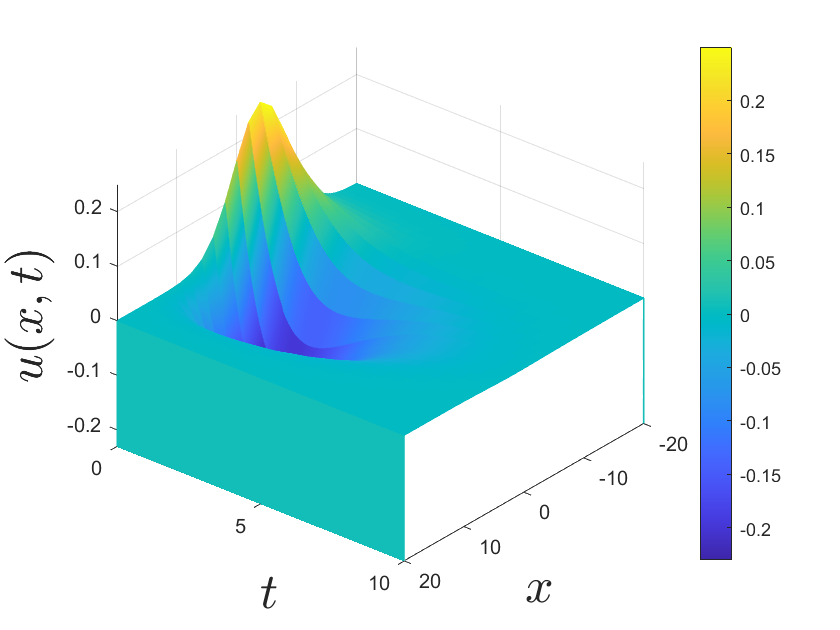
\includegraphics[scale = 0.35]{scicompProb3u}
    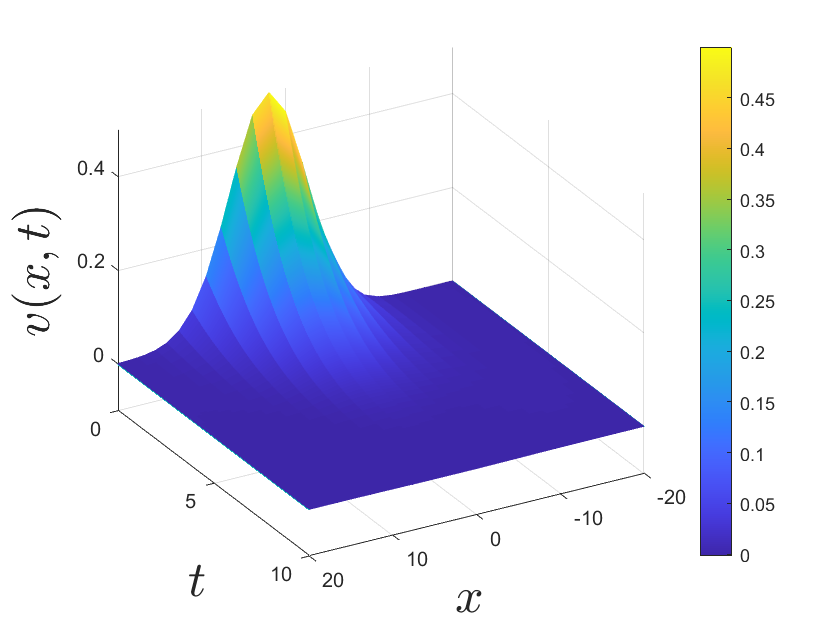
\includegraphics[scale = 0.35]{scicompProb3v}
    \newline
    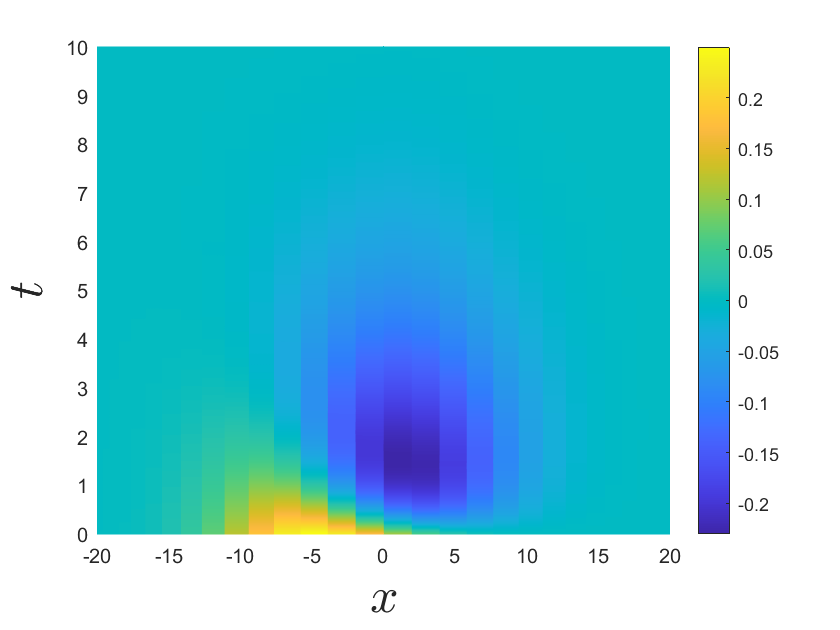
\includegraphics[scale = 0.35]{scicompProb3utop}
    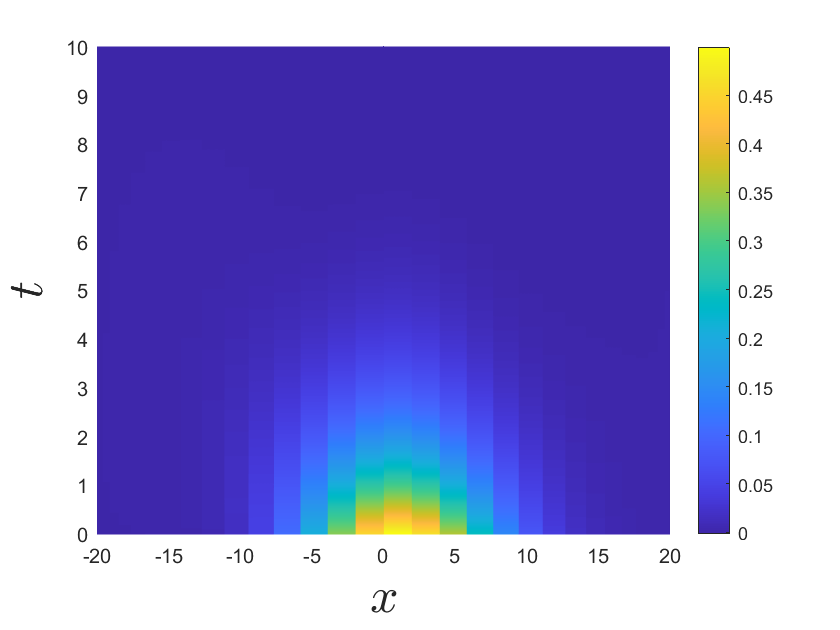
\includegraphics[scale = 0.35]{scicompProb3vtop}
\end{center}
See attached \verb+scicompMidterm3_NAMEIKA+ script.

\end{document}
